\chapter{Completed Work}

We have developed a prototype of a visualization for the MS-PROD model in C++ using OpenGL, built on top of the C++ and Qt code provided by the MS-PROD authors.  Standard line charts---of both the simple line chart and small multiples varieties---were chosen to display the biomass forecast data outputted by the model.  A major reason line charts were chosen is that casual viewers can understand them without further instructions, as opposed to a horizon graph.  Another advantage to line charts is that they tend to have a reasonable amount of whitespace where additional information can be displayed, such as uncertainty or alternate forecasts.

The MS-PROD application is started by selecting an input parameter file in CSV format specifying the initial biomass, growth rate, catchability, predation, and interaction values for each species.  The output of the model is displayed on line charts, with time on the $x$-axis and biomass on the $y$-axis.  The user can adjust sliders which represent harvest effort and watch the line charts change instantaneously as the model is re-run according to the new effort values.  Like Eberlein and Peterson, we aimed to turn the ``time consuming and tedious'' task of working with a model into a ``fast and fun'' interactive experience \cite{eberlein1992}.  Different views and features of the visualization are discussed in the sections below.  

\section{Functional Group View}

\begin{figure}[h]
	\centering
	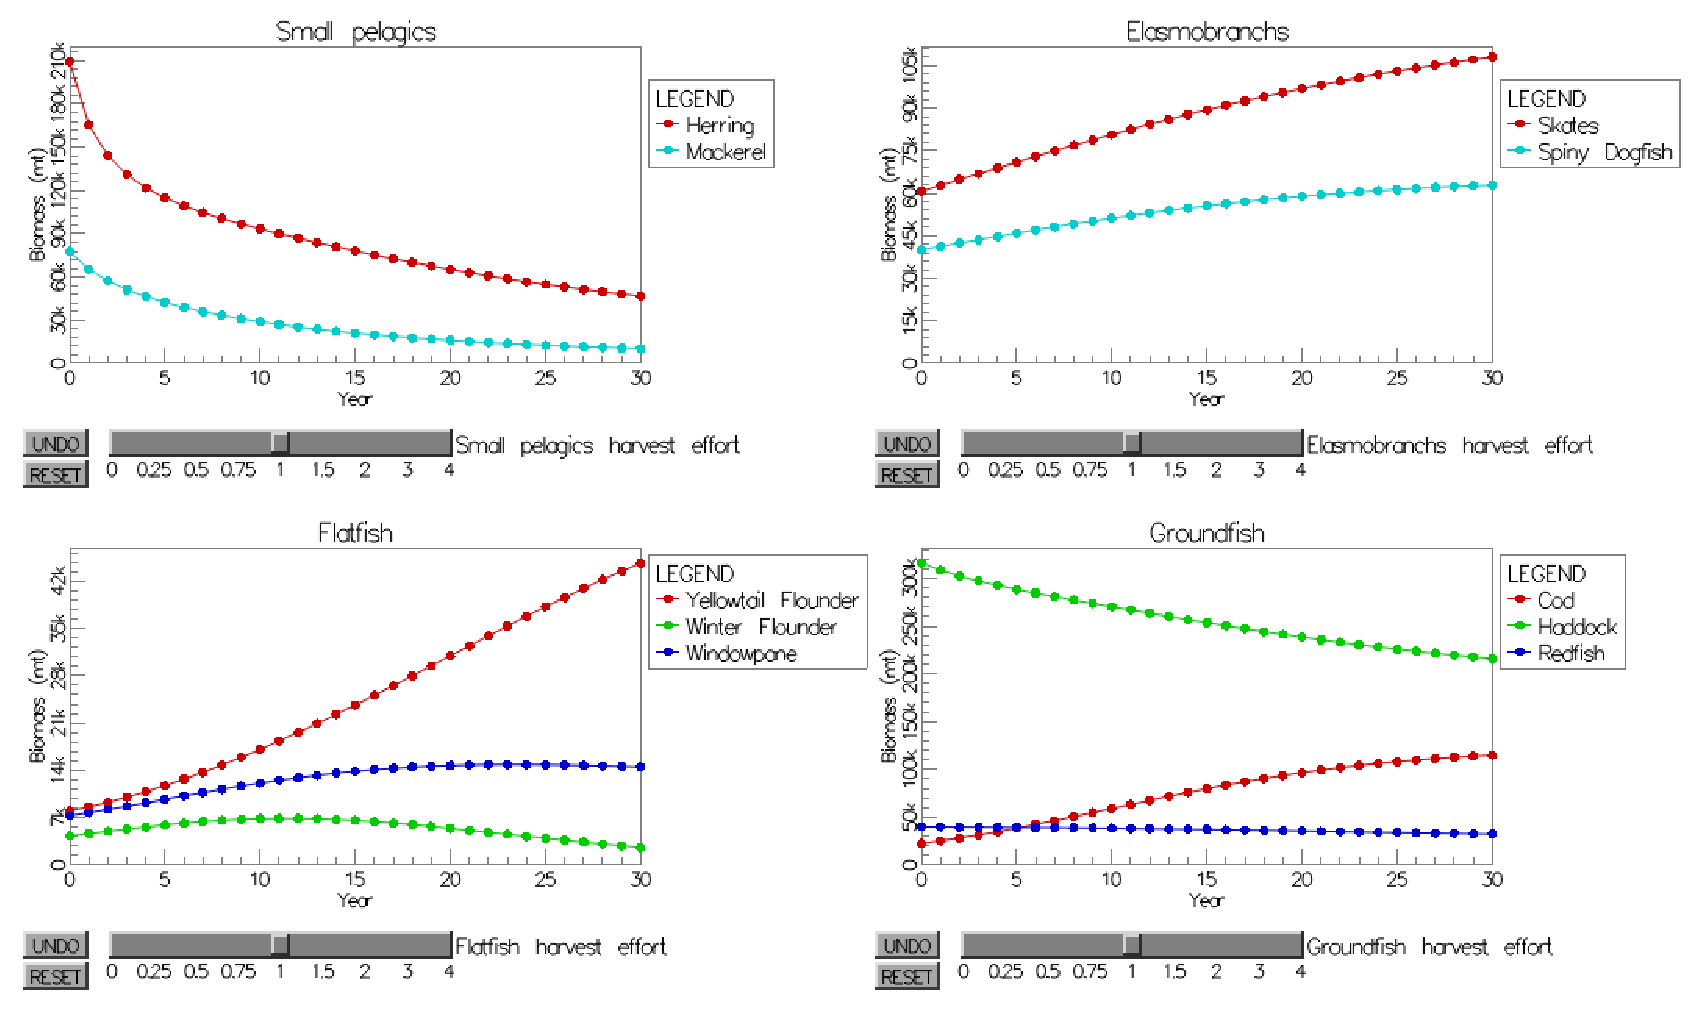
\includegraphics[width=15cm]{figures/eps/msprod_group.eps}
	\caption{A ``by group'' view of our MS-PROD visualization.}
	\label{fig:msprod_group}
\end{figure}

Initial attempts to display all species on a single line chart proved to be ineffective; apart from the problem of selecting enough distinct colors to represent each species, the biomass of some species was significantly larger than others.  By scaling the $y$-axis according to the largest biomass value in the entire 30-year timespan, the lines representing some species were crowded at the bottom of the chart and seemed to be flat even when they were not.  It was observed that species of similar functional groups tend to have biomass values in similar numeric ranges.  Combined with the fact that harvest effort is controlled by functional group, it made sense to develop a line chart for each functional group.

A functional group is a biological grouping of species which perform similar functions within their ecosystem---e.g., mackeral and herring are both members of the ``small pelagic'' group since they live in the water column.  The MS-PROD model requires that the functional group of each species is specified in the input parameter file; the four featured in the input file used for the majority of the development were small pelagics, elasmobranchs, flatfish, and groundfish.  Figure~\ref{fig:msprod_group} shows a screenshot of biomass predictions produced by the model and displayed by these four functional groups.

The major advantage of this ``by group'' view is that comparisons of species within a group are easy.  For MS-PROD, there are only two or three species per functional group, so the line chart for each group tends to not suffer from occlusion problems, unlike with the initial single line chart approach.  Direct and indirect effects of changes in harvest effort also become more clear with the ``by group'' approach---e.g., if the user adjusts the effort slider only for elasmobranchs, yet sees the biomasses change on the groundfish chart, then the user can begin to understand there is some kind of relationship between elasmobranchs and groundfish.

\section{Species View}

\begin{figure}[h]
	\centering
	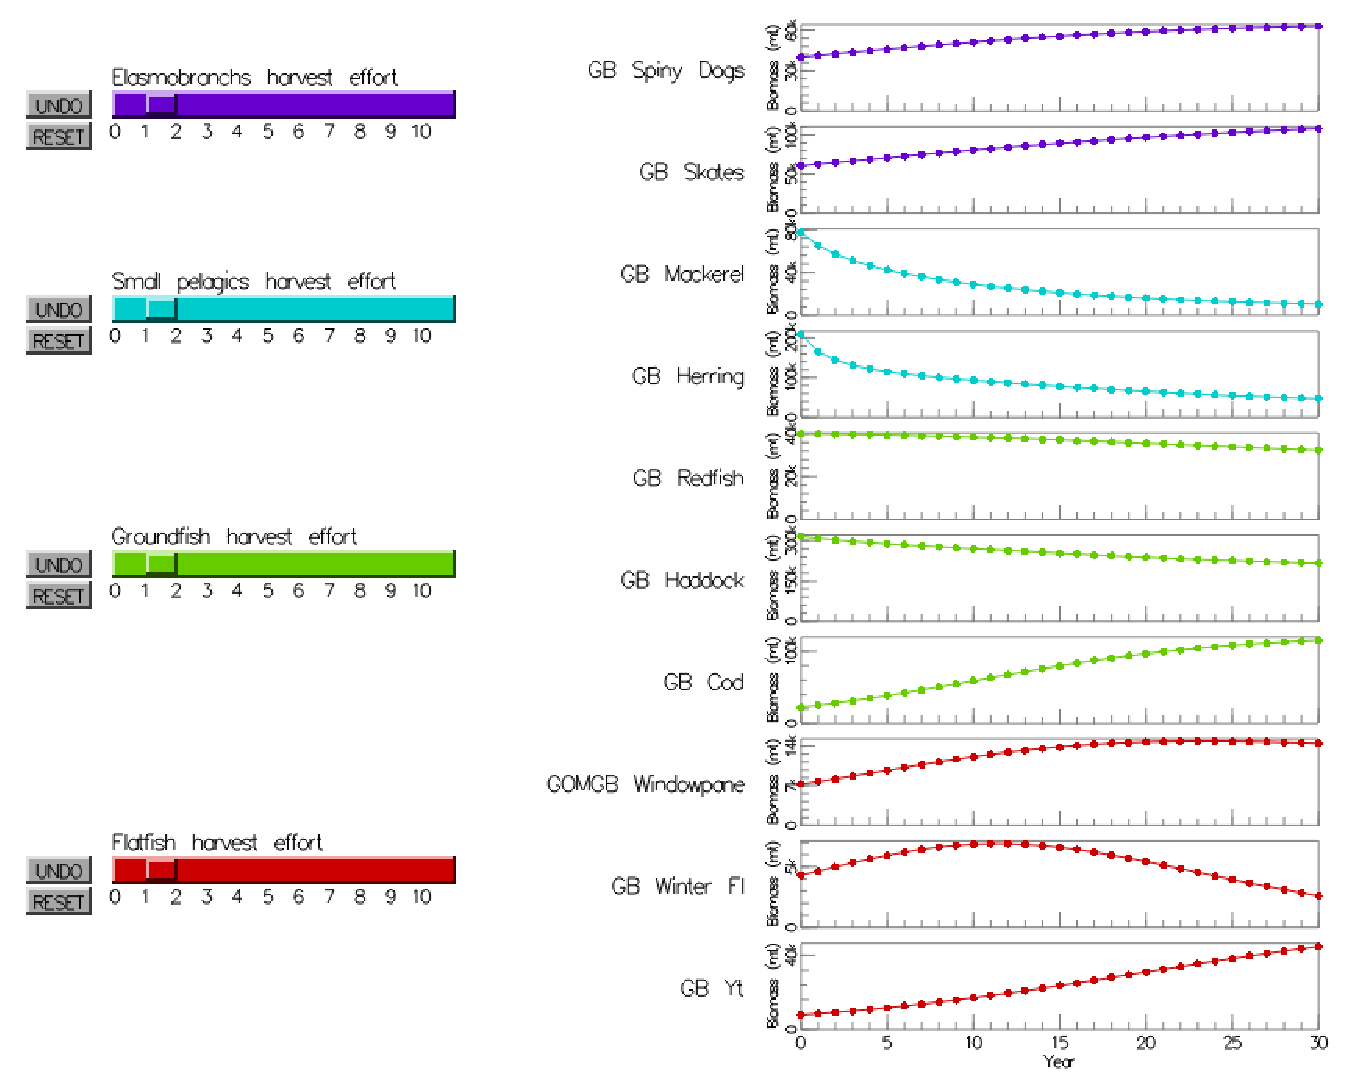
\includegraphics[width=13cm]{figures/eps/msprod_species.eps}
	\caption{A ``by species'' view of our MS-PROD visualization.}
	\label{fig:msprod_species}
\end{figure}

The alternative to viewing ``by group'' is to view each species on its own plot, as in small multiples.  In this style, each plot is sorted and colored according to functional group membership, as seen in Figure~\ref{fig:msprod_species}.  The harvest effort sliders are also colored by functional group and positioned near the plots of the corresponding group.  This allows for the ability to differentiate between direct and indirect effects of changes in harvest effort.

With each species on its own plot, it is much easier to interpet the biomass predictions of an individual species, since the $y$-dimension of a plot needs to be scaled to the data of one species only.  It is easier to perceive increases or decreases in biomass because no species suffers from the flattening that can occur when a series is displayed on the same plot as a series that has significantly higher values.  On the other hand, this makes comparison between species somewhat difficult because the user must either refer to the $y$-axis labels or hover over a specific point on a chart in order to determine the absolute value of the biomass at a point in time.

\subsection{Absolute Size Indicators}

In the ``by-species'' view, the scaling of the $y$-dimension is adjusted to fit the data of each chart.

\subsection{Between Species Arcs}

\subsection{Predation}

\subsection{Interaction}

\section{Displaying Change}

